\section{Anatomy of an LLM-based Agent}
\label{sec:agent-anatomy}

An LLM-based agent is built around a small set of recurring components: tool use, memory, and planning. Tool use is the defining component, since it extends the language model from a system that emits text to one that can act on its environment. Together, these components produce the trajectory, the ordered sequence of reasoning steps, tool calls, and intermediate outputs that the agent goes through before it returns a final response. The trajectory is the unit on which later evaluation operates.

\subsection{The ReAct loop}
\label{subsec:tool-use-react}

ReAct, short for reasoning and acting, is a method that connects language models to the classical notion of an autonomous agent, later turned into a first-class abstraction by the function-calling interface of Section~\ref{sec:structured-output} \cite{yaoReActSynergizingReasoning2022, FunctionCallingOther2024}. The method described in the paper consists of a prompting technique that prompts the model to generate reasoning traces and task-specific actions in an interleaved manner. On the two interactive decision-making benchmarks ALFWorld and WebShop, it improved the absolute success rate over imitation and reinforcement learning baselines by 34\% and 10\% respectively, while using only one or two in-context examples \cite{yaoReActSynergizingReasoning2022}. The action space is augmented to
\begin{equation}
    \hat{A} = A \cup L,
\end{equation}
where
\begin{itemize}
    \item $A$ is the set of domain actions;
    \item $L$ is the space of language \cite{yaoReActSynergizingReasoning2022}.
\end{itemize}
$L$ is the language the model produces as output. An action drawn from $L$, called a thought, does not affect the environment and produces no observation: it lets the model induce, track, and update plans, handle exceptions, and compose information by reasoning over the current context, updating that context for the steps that follow \cite{yaoReActSynergizingReasoning2022}. An action drawn from $A$ interfaces with an external source, such as a weather API, and returns information into the context. In the original formulation, a frozen language model is prompted with few-shot examples to emit both thoughts and actions, producing a trajectory of interleaved thought, action, and observation steps, with no runtime component beyond the prompt \cite{yaoReActSynergizingReasoning2022}. Figure~\ref{fig:react-example} shows such a trajectory for a query about the weather in the user's city, where the model first retrieves the city and then queries the weather for it.

\begin{figure}[ht]
	\centering
	\vspace{4mm}
	\begin{tikzpicture}[
		node distance=5mm,
		every node/.style={font=\small},
		thought/.style={draw, dashed, rounded corners, align=left, text width=0.82\textwidth, inner sep=5pt},
		action/.style={draw, rounded corners, align=left, text width=0.82\textwidth, inner sep=5pt},
		obs/.style={align=left, text width=0.82\textwidth, inner sep=5pt, font=\small\itshape},
		query/.style={draw, thick, rounded corners, align=left, text width=0.82\textwidth, inner sep=5pt, font=\small\bfseries},
		arr/.style={-{Latex[length=2mm]}}
		]
		\node[query] (q) {Query: What is the weather in my city?};
		\node[thought, below=of q] (t1) {[L] Thought 1: The query asks for the weather in the user's city, but the city is not in the context. I should look it up first.};
		\node[action, below=of t1] (a1) {[A] Action 1: \texttt{get\_location[]}};
		\node[obs, below=of a1] (o1) {Observation 1: city is London};
		\node[thought, below=of o1] (t2) {[L] Thought 2: The city is London. Now I can check the weather for it.};
		\node[action, below=of t2] (a2) {[A] Action 2: \texttt{get\_weather[London]}};
		\node[obs, below=of a2] (o2) {Observation 2: 22\textdegree C, partly cloudy};
		\node[thought, below=of o2] (t3) {[L] Thought 3: The weather in London is now known, so the query can be answered.};
		\node[action, below=of t3] (a3) {[A] Action 3: \texttt{finish[22\textdegree C, partly cloudy in London]}};
		\foreach \x/\y in {q/t1, t1/a1, a1/o1, o1/t2, t2/a2, a2/o2, o2/t3, t3/a3}
			\draw[arr] (\x) -- (\y);
	\end{tikzpicture}
	\caption[An example ReAct trajectory for a weather query]{An example ReAct trajectory for a weather query.}
	\label{fig:react-example}
\end{figure}

In the function-calling interface, each action of Figure~\ref{fig:react-example} becomes a declared function call, such as \texttt{get\_weather(city="London")}, and each observation becomes the value the runtime returns. This interface is architecturally similar to the thought, action, and observation cycle of ReAct, but it separates the concerns of the cycle. The model first declares intent by selecting a function and its arguments, then the runtime executes the call, and the result is injected back into the context as the next input. ReAct couples the generation of the action and its execution within the prompt and the surrounding environment, but function calling assigns execution to the runtime and leaves the model responsible only for declaring the call. Figure~\ref{fig:react-loop} shows the loop as implemented with function calling.

\begin{figure}[ht]
	\centering
	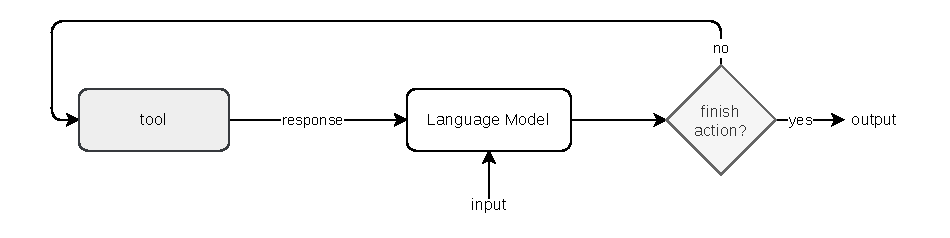
\includegraphics[width=0.92\textwidth]{images/react_loop.pdf}
	\caption[The ReAct loop with tool calling]{The ReAct loop with tool calling}
	\label{fig:react-loop}
\end{figure}

This loop matches the perceive-decide-act cycle of the classical agent of Section~\ref{sec:classical-agent}. The model carries out the decide step; the environment executing a call realizes the act step; the returned response supplies the perceive step. Table~\ref{tab:classical-llm} extends the same correspondence to every component, mapping the elements of the formulation of Russell and Norvig onto their counterparts in an LLM-based agent.
\begin{table}[ht]
	\centering
	\small
	\begin{tabularx}{\textwidth}{@{}XX@{}}
		\toprule
		Classical agent & LLM-based agent \\
		\midrule
		Percept & Content entering the context, including tool results \\
    Actions & Tool calls \\
		Agent function & A forward pass of the language model \\
		Internal state & Context window \\
		Performance measure & External evaluation criterion, applied after the run \\
		\bottomrule
	\end{tabularx}
	\caption[Correspondence between classical agent and LLM-based agents]{Correspondence between classical agent and LLM-based agents.}
	\label{tab:classical-llm}
\end{table}

The performance measure of Section~\ref{subsec:rationality} drives action selection during the run, since the decide step selects the action expected to maximize it \cite[Chap.~2]{russellArtificialIntelligenceModern2022}. An LLM-based agent has no such measure active during the run. It is not built for one task and its objective is defined in the prompt as natural language; therefore, no criterion over states is available to it while it runs. The criterion is applied only after the run, by an evaluation setup that decides both what to evaluate and how to evaluate it \cite{mohammadiEvaluationBenchmarkingLLM2025}. Chapter~\ref{chap:evaluating-agents} describes how such a criterion is defined.

\subsection{Building blocks}
\label{subsec:building-blocks}

So far, the minimal agent has been defined by a language model, a set of tools, and the loop that connects them. On a higher level of abstraction, the loop and the tool definitions allow the agent to be described as a set of components organized around the language model. Zhao et al. and Wang et al. converge on the same three: memory, planning, and an execution component that carries out the plan, called action by Wang et al. \cite{zhaoSurveyLargeLanguage2026, wangSurveyLargeLanguage2024}. Zhao et al. describe the language model as the core computation unit, equipped with these three components and integrated under its control during interactions with the environment \cite{zhaoSurveyLargeLanguage2026}. Wang et al. add a fourth module, profiling, which identifies the role of the agent and influences the memory and planning modules; those two modules, together with profiling, in turn influence the action module \cite{wangSurveyLargeLanguage2024}. The three shared modules are described below. The ReAct loop of Section~\ref{subsec:tool-use-react} sequences their use.

\paragraph{Planning.} The planning component decomposes a complex task into simpler subtasks that are solved individually \cite{wangSurveyLargeLanguage2024}. Wang et al. separated existing designs according to whether the agent receives feedback during the planning process \cite{wangSurveyLargeLanguage2024}:
\begin{itemize}
    \item \emph{Planning without feedback}, where the agent does not receive feedback that can influence its future behavior after taking actions. This covers single-path reasoning, in which the task is decomposed into intermediate steps connected in a pipeline, each leading to a single subsequent step. It also covers multi-path reasoning, in which the steps are organized into a tree and each step may have several subsequent steps, and the delegation of plan generation to a well-developed external planner \cite{wangSurveyLargeLanguage2024}.
    \item \emph{Planning with feedback}, where the agent revises its plans after taking actions on the basis of signals obtained from the environment, from humans, or from a model. This is better suited to complex tasks that need long-horizon planning, where planning without feedback is less effective \cite{wangSurveyLargeLanguage2024}.
\end{itemize}

\paragraph{Memory.} The memory component stores information perceived from the environment and uses the recorded memories to facilitate future actions \cite{wangSurveyLargeLanguage2024}. Wang et al. analyzed it along three perspectives \cite{wangSurveyLargeLanguage2024}:
\begin{itemize}
    \item \emph{Structures}, which distinguish short-term from long-term memory. Short-term memory consists of the information within the context window constrained by the transformer architecture, while long-term memory resembles an external store that the agent can query and retrieve from as needed.
    \item \emph{Formats}, the medium in which the content is stored, including raw natural language, embedding vectors, databases, and structured lists \cite{wangSurveyLargeLanguage2024}.
    \item \emph{Operations}, through which the component interacts with the environment: \textbf{reading}, which extracts relevant information from memory to inform the next action; \textbf{writing}, which stores new information while handling duplication and storage limits; and \textbf{reflection}, which summarizes past records into higher-level insights \cite{wangSurveyLargeLanguage2024}.
\end{itemize}

\paragraph{Action.} The action component translates the agent's decisions into specific outcomes and is located at the most downstream position, where it directly interacts with the environment \cite{wangSurveyLargeLanguage2024}. Two of the perspectives used by Wang et al. bear on the runtime structure \cite{wangSurveyLargeLanguage2024}:
\begin{itemize}
    \item The \emph{action space}, the set of actions available to the agent, divided into external tools and what the model already knows from training. External tools include APIs, databases and knowledge bases, and other models, each of which expands the action space beyond the limitations of the language model on its own \cite{wangSurveyLargeLanguage2024}.
    \item The \emph{action impact}, the consequence of an action, which may change the environment, alter the agent's own internal state such as its memory or plans, or trigger further actions \cite{wangSurveyLargeLanguage2024}.
\end{itemize}

Systems with more than one specialized function add a routing mechanism. It governs the flow of control to different specialized functions, tools, or sub-processes. Through it, the agent evaluates specific criteria and selects from a set of possible subsequent actions instead of following a fixed execution path \cite[Chap.~2]{gulliAgenticDesignPatterns2025}.

Figure~\ref{fig:agent-blocks} shows the complete agent: the language model receives an input and produces a response, drawing on planning and memory and issuing tool calls that act on the environment.

\begin{figure}[ht]
	\centering
	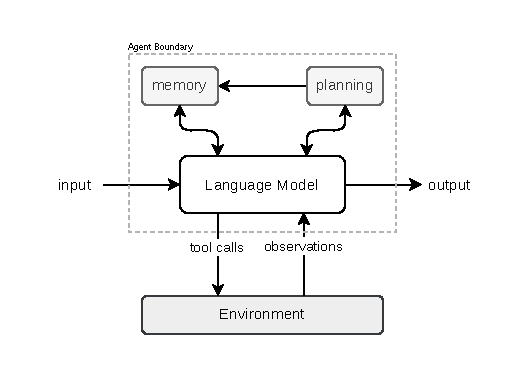
\includegraphics[width=0.75\textwidth]{images/agent_blocks.pdf}
	\caption[The complete LLM-based agent with its building blocks]{The complete LLM-based agent with its building blocks}
	\label{fig:agent-blocks}
\end{figure}

\subsection{Memory and retrieval}
\label{subsec:memory-reml}

The long-term part of the memory component rests on information retrieval. Wang et al. distinguished a unified structure from a hybrid structure \cite{wangSurveyLargeLanguage2024}. A unified structure holds only the short-term memory of Section~\ref{subsec:building-blocks}, directly in the context window. A hybrid structure adds long-term memory: it retrieves relevant records from an external store and inserts them into the prompt, governed by the reading operation and its relevance scoring \cite{wangSurveyLargeLanguage2024}. Retrieval-augmented generation implements this scheme by retrieving relevant information from an external knowledge base, which reduces the generation of factually incorrect content and allows continuous knowledge updates and the integration of domain-specific information \cite{gaoRetrievalAugmentedGenerationLarge2024}. Retrieval introduces failure modes of its own: low precision leads to the selection of misaligned or irrelevant content, and low recall leads to missing crucial information \cite{gaoRetrievalAugmentedGenerationLarge2024}. The model may still produce content not supported by the retrieved context, and it may echo retrieved content without synthesizing it \cite{gaoRetrievalAugmentedGenerationLarge2024}. What enters the context through memory affects every subsequent step, so an error in retrieval propagates through the rest of the loop.

\subsection{Role and configuration}
\label{subsec:agent-identity}

Section~\ref{subsec:new-decide-step} shows that constructing a new agent means changing the prompt, the tools, and the retrieved context, not the model itself. Multiple agents can therefore share the same underlying model and still be told apart, which raises the question of what distinguishes one agent from another, and of whether an agent whose prompt or toolset has changed still counts as the same agent.

The profiling module of Section~\ref{subsec:building-blocks} identifies an agent by its \emph{role}, such as planner, speaker, coordinator, or specialist, written into the prompt to shape the model's behavior \cite{wangSurveyLargeLanguage2024}. Wang et al. use this to populate a system with several distinct agents, for example assigning software-development roles to a collaborating team or generating a population of agents for social simulation \cite{wangSurveyLargeLanguage2024}. In their examples, the role is what tells two agents in the same system apart.

The role and the configuration answer this at two different levels of abstraction, and the two coexist:

\begin{itemize}
	\item At a higher level of abstraction, an agent is defined by the role it occupies, and stays the same agent across a change to its configuration, as long as it keeps the same role.
	\item At a lower level of abstraction, an agent is defined by the prompt, the underlying model, and the toolset made available to it.
\end{itemize}
